\section{Classification and regression}\label{sec:m3}

\subsection{Experimental design}
The target is \attr{seller\_rating\_class}, predicted from the 19 numerical and 5 categorical attributes of \cref{sec:corr}. One stratified 80/20 split (11\,074 / 2\,769 sellers, seed 42) is shared by every classifier, by the regressions and by the rules of \cref{sec:exploit}. All tuning uses stratified 5-fold CV on the training set, with imputation, log, scaling, encoding and binning refitted \emph{inside} each fold. We select by \textbf{macro-F1}, which weighs the three classes equally; the majority class scores 0.236 (accuracy 0.547), stratified random guessing 0.334. The way to handle imbalance is itself a hyperparameter of each model.

\subsection{Baseline grids}\label{sec:grids}
\Cref{tab:grids} lists all tested values (658 configurations), with the best CV macro-F1 each value reaches.

\begin{table*}[t]
\centering
\caption{Baseline grids: tested values, each followed by the best CV macro-F1 over the rest of the grid (bold: chosen).}\label{tab:grids}
{\tabfont\setlength{\tabcolsep}{4pt}
\begin{tabular}{@{}l l p{0.655\textwidth}@{}}
\toprule
Model (configs) & Parameter & Values (best CV macro-F1)\\
\midrule
Decision Tree (432) & criterion & \textbf{gini} .419, entropy .406\\
 & max depth & 2 .392, 3 .395, 4 .367, \textbf{5} .419, 6 .411, 8 .409, 10 .412, 12 .411, none .411\\
 & min samples leaf; split & leaf: 1 .417, 5 .417, 20 .419, \textbf{50} .419; split: \textbf{2}, 20, 100 all .419\\
 & class weight & none .407, \textbf{balanced} .419\\
\midrule
KNN (128) & $k$ & 1 .390, 3 .388, 5 .392, 7 .387, 9 .392, 11 .402, 15 .409, 21 .415, 31 .416, 41 .424, 51 .424, 75 .429, 101 .434, \textbf{151} .434, 201 .433, 301 .429\\
 & Minkowski $p$; weights & $p$: \textbf{1} .434, 2 .434; weights: uniform .432, \textbf{distance} .434\\
 & decision rule & plain vote .390, \textbf{prior-corrected} .434\\
\midrule
GaussianNB (26) & var.\ smoothing; priors & $10^{-12}$--$10^{-3}$ .403, $10^{-2}$ .403, $\mathbf{10^{-1}}$ .404, 1 .400; priors: empirical .391, \textbf{uniform} .404\\
CategoricalNB (72) & bins; $\alpha$; priors & bins: \textbf{3} .416, 4 .413, 5 .412, 6 .414, 8 .412, 10 .412; $\alpha$: \textbf{0.01}--5 all .415--.416; priors: \textbf{empirical} .416, uniform .404\\
\bottomrule
\end{tabular}}
\end{table*}

\paragraph{Decision Tree} Inputs are not scaled (splits are invariant). Depth and class weighting matter; criterion and minimum split size hardly do. \Cref{tab:prune,fig:overfit} show overfitting control: the unpruned tree (3\,350 leaves) memorizes the training set (F1 1.00) and reaches 0.387 in CV; pre-pruning at depth 5 (31 leaves) gives 0.419 with a small gap. Cost-complexity pruning (40 $\alpha$ values along the pruning path) peaks at $\alpha=4.5\cdot10^{-4}$, with 93 leaves, and stays below (0.401). The depth curve has a dip at 4 and a flat tail, so it reads ``shallow is enough'' and not ``exactly 5''.

\begin{table}[t]
\centering
\caption{Unpruned vs pre- and post-pruned tree.}\label{tab:prune}
\tab{m3_prune}
\end{table}

\begin{figure*}[t]
\centering
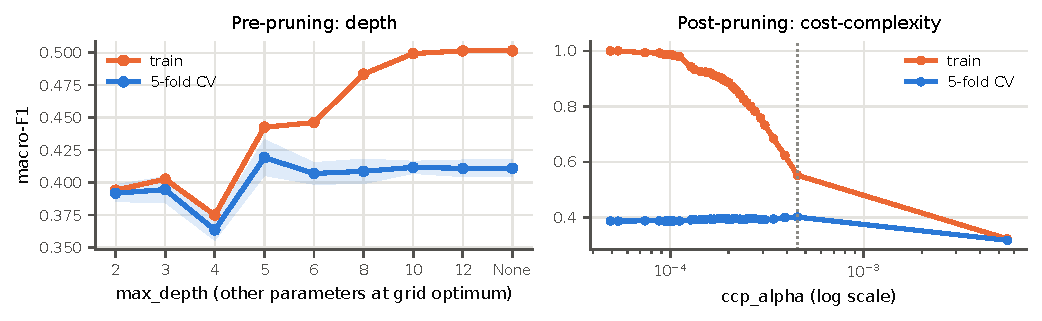
\includegraphics[width=0.93\textwidth]{m3_dt_overfitting}
\caption{Decision Tree: train and CV macro-F1 vs depth (left) and cost-complexity $\alpha$ (right).}\label{fig:overfit}
\end{figure*}

\paragraph{KNN} It works on log, standardized, one-hot data. With the plain vote, macro-F1 falls from 0.38 to 0.24 as $k$ grows while accuracy rises to the majority level (\cref{fig:knn}): large neighbourhoods always contain more \emph{medium} sellers. The prior-corrected rule $\arg\max_c P(c\mid x)/P(c)$ reverses the trend, with a plateau for $k=101$--$201$. Metric and weighting are secondary. The training F1 of 1 under distance weights is trivial (each point is its own nearest neighbour) and is not a sign of overfitting.

\begin{figure*}[t]
\centering
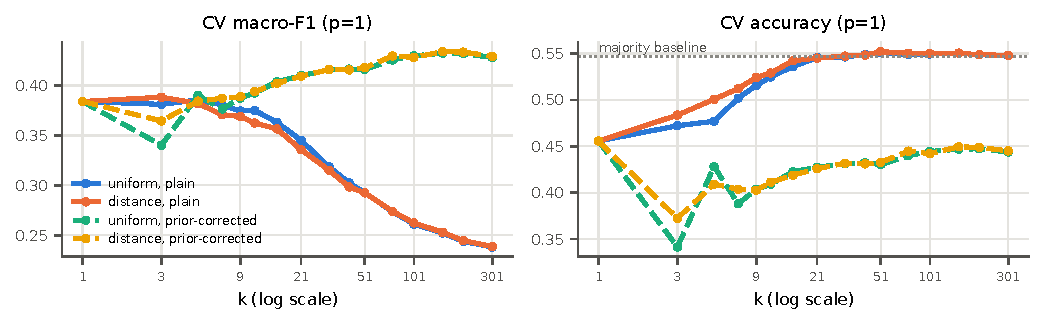
\includegraphics[width=0.93\textwidth]{m3_knn_k}
\caption{KNN: CV macro-F1 (left) and accuracy (right) vs $k$, by weighting and decision rule.}\label{fig:knn}
\end{figure*}

\paragraph{Na\"ive Bayes} GaussianNB uses the 19 numerical attributes, log-transformed and standardized. Scaling matters although the model is scale-invariant in theory: \code{var\_smoothing} adds a fraction of the largest variance to all variances, and unscaled mileage flattened all other attributes (0.31). CategoricalNB uses all 24 attributes, with quantile bins; three coarse bins are best and $\alpha$ is irrelevant (hundreds of sellers per bin). Both assumptions are violated: within each class $\rho_s$(mileage, share of new) is $-0.81$ to $-0.87$ and $\rho_s$(hp, tank) is about 0.8, and 11 of 19 attributes keep $|\mathrm{skew}|>1$ in some class. Correlated evidence is counted several times, which hurts probabilities more than rankings; binning removes the Gaussian assumption, hence CategoricalNB's edge.

\subsection{Baseline results on the test set}\label{sec:test}
\begin{table*}[t]
\centering
\caption{Test set, baseline-grid models: overall metrics and precision/recall/F1 per class (best of each grid by CV macro-F1).}\label{tab:test}
\tabtight{m3_test}
\end{table*}

\begin{figure*}[t]
\centering
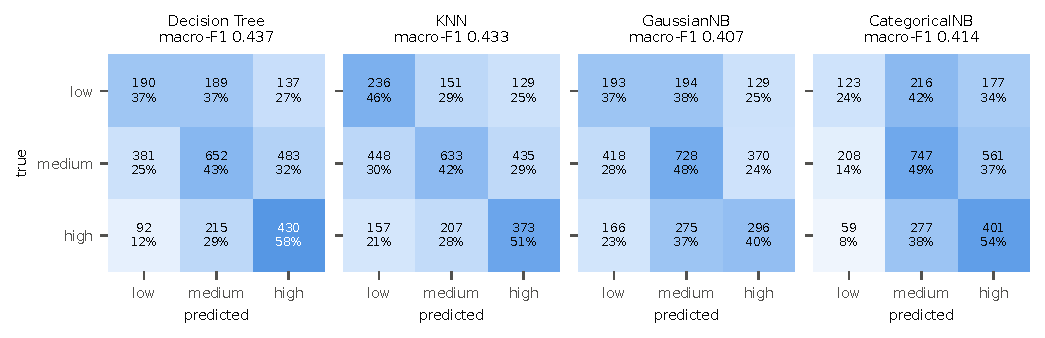
\includegraphics[width=0.95\textwidth]{m3_confusion}
\caption{Confusion matrices on the test set (counts and row percentages).}\label{fig:conf}
\end{figure*}

\begin{figure*}[t]
\centering
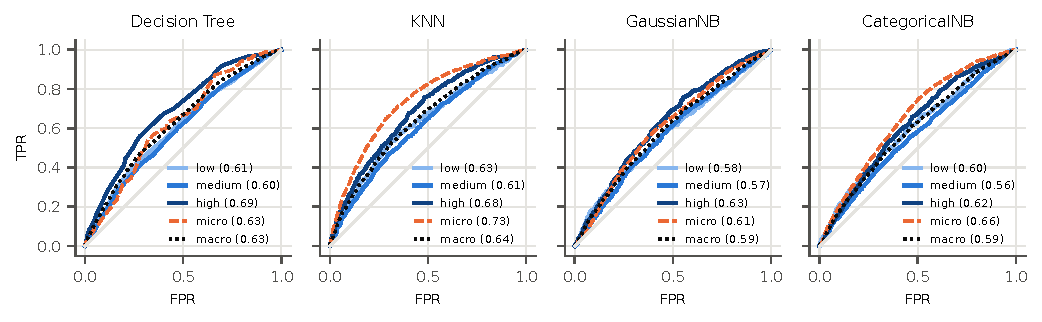
\includegraphics[width=0.95\textwidth]{m3_roc}
\caption{One-vs-rest ROC curves with per-class, micro and macro AUC (test set).}\label{fig:roc}
\end{figure*}

All models (\cref{tab:test}) clearly beat the majority class in macro-F1 (0.41--0.44 vs 0.24) and, as expected when all classes weigh the same, stay below its accuracy. CV and test scores differ by at most 0.02. The Decision Tree and KNN lead; the tree has the best \emph{high} recall (0.58), KNN the best \emph{low} recall (0.46) and the best AUC (macro 0.64, micro 0.73), since a 151-neighbour frequency is a smooth score while the tree only outputs 31 distinct values (stepped curves in \cref{fig:roc}). In \cref{fig:conf} \emph{medium} leaks to both sides: the tree sends 25\% of it to \emph{low} and 32\% to \emph{high}. \emph{High} is the easiest class for every model (AUC 0.62--0.69); CategoricalNB finds only 24\% of \emph{low}. An AUC of 0.6 means that the attributes rank sellers only slightly better than chance, which motivates the experiments below.

\subsection{Sensitivity of the baselines}\label{sec:ablation}
Before improving the models we asked what they depend on. Each row of \cref{tab:abl} changes one element of a baseline and repeats the same 5 folds (everything refitted inside the folds, the test set untouched).

\begin{table}[t]
\centering
\caption{Ablations: change of CV macro-F1 vs the baseline on identical folds. Bold: same sign in all five folds. Trees are invariant to scale.}\label{tab:abl}
\tab{m5_ablation}
\end{table}

\begin{itemize}
\item \textbf{Scale} is decisive for distances: unscaled KNN loses 0.063 and unscaled GaussianNB 0.097, because mileage and price dominate. The log matters less (0.003 and 0.014); standardization beats min--max and robust scaling, which are distorted by extremes or by zero-inflated attributes.
\item \textbf{Outliers}: winsorizing changes nothing, and removing DBSCAN noise from the training folds \emph{hurts} all models ($-0.010$ to $-0.018$). The extreme sellers carry information, which supports keeping them (\cref{sec:quality}).
\item \textbf{Attributes}: seller size and the block price--turnover--wear are needed; vehicle specifications, 8 of the 19 numerical attributes, contribute nothing to the tree and KNN. Size alone gives only 0.36.
\item \textbf{Segments as features} help the tree slightly ($+0.006$, all folds) and hurt KNN and GaussianNB, where they duplicate existing distances.
\end{itemize}

\subsection{Extended models: partial prior correction and engineered attributes}\label{sec:tau}
\paragraph{Idea} The baselines treat imbalance as all or nothing: no correction ignores the minority classes, full balancing sends half of \emph{medium} elsewhere. We interpolate with an exponent $\tau$:
\begin{equation}
\hat y=\arg\max_c \frac{P(c\mid x)}{P(c)^{\tau}},\qquad \tau\in[0,1].
\end{equation}
$\tau=0$ is the plain rule and $\tau=1$ the prior-corrected rule of KNN. For the tree the same exponent defines the class weights $w_c\propto P(c)^{-\tau}$ ($\tau=1$ is \code{balanced}), for Na\"ive Bayes it rescales the prior. We added 12 attributes computed from a seller's own row, so they cannot leak: listings per active day, share of active days, listing rate, savings/price, number of new, used, theft, salvage and ex-taxi vehicles, price per hp, miles per year, days on market over span.

\paragraph{Search} $\tau\in\{0,.25,.5,.6,.7,.8,.9,1\}$ and engineered attributes on/off, crossed with: tree depth $\{4,5,6,8,10\}$ and leaf $\{20,50,100\}$; KNN $k\in\{51,101,151,201\}$ (distance weights, $p=1$); GaussianNB smoothing $\{10^{-3},10^{-2},10^{-1}\}$; CategoricalNB bins $\{3,4,6\}$: 400 configurations. Intermediate $\tau$ wins clearly for the tree ($\tau=0.7$, 0.445 vs 0.419 at 1) and KNN ($\tau=0.8$, 0.456 vs 0.438), while Na\"ive Bayes is flat (\cref{fig:tau}, left): its over-confident posteriors are barely moved by a prior factor. Chosen: tree with depth 4, leaf 20, $\tau=0.7$; KNN with $k=151$, $\tau=0.8$; GaussianNB with smoothing $10^{-3}$, $\tau=0$; CategoricalNB with 4 bins, $\tau=0$; all with engineered attributes.

\begin{figure*}[t]
\centering
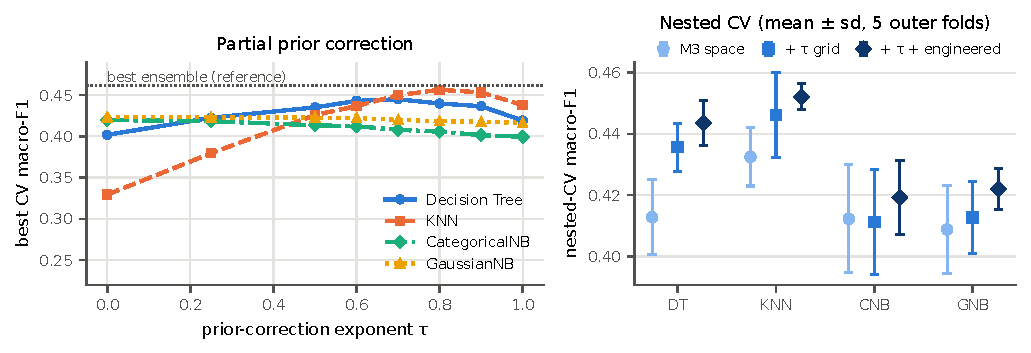
\includegraphics[width=0.93\textwidth]{m5_tau}
\caption{Left: best CV macro-F1 for each value of $\tau$. Right: nested CV of the three search spaces.}\label{fig:tau}
\end{figure*}

\paragraph{Nested CV} Larger grids look better by chance, so we compared whole search spaces with \emph{nested} CV (inner 5-fold search, outer 5-fold score; \cref{tab:nested}). The $\tau$ grid improves tree and KNN in all five folds and the engineered attributes add a little more: $+0.031$ for the tree and $+0.020$ for KNN in total. Na\"ive Bayes gains only from the attributes (about $+0.01$).

\begin{table}[t]
\centering
\caption{Nested CV macro-F1 (mean$\pm$sd; folds better than the baseline space in brackets).}\label{tab:nested}
\tabtight{m5_nested}
\end{table}

\paragraph{Test set} The test set had been used once for the baselines (\cref{tab:test}); here it is used once more, for the single configuration per model fixed by CV. \Cref{tab:ext,fig:ci} add bootstrap confidence intervals (2\,000 resamples of the test sellers). Two ensembles outside the lecture programme (a 300-tree random forest and gradient boosting, only $\tau$ tuned) are a yardstick, not candidates. Paired bootstrap on the same resamples:
\begin{itemize}
\item the baseline tree, KNN and the rules of \cref{sec:exploit} are tied (all intervals of the differences contain 0 and lie within $\pm0.025$), while the tree beats GaussianNB (CI $[0.006,0.052]$);
\item extended KNN beats baseline KNN by 0.031, CI $[0.013,0.047]$; the extended tree gains 0.007, not significant ($[-0.011,0.025]$), although its CV gain was larger: the baseline tree had been lucky on the test set (CV 0.419, test 0.437);
\item extended KNN is ahead of the extended tree by 0.020, $[0.000,0.041]$, and level with gradient boosting ($[-0.015,0.018]$) and the random forest ($[-0.004,0.027]$).
\end{itemize}
A partial correction also restores accuracy (0.45 to 0.52 for KNN), because fewer \emph{medium} sellers are sacrificed. The price is a lower \emph{low} recall (0.46 to 0.27 for KNN, 0.37 to 0.19 for the tree). For KNN the F1 of \emph{medium} (0.505 to 0.608) and \emph{high} (0.446 to 0.486) rises and that of \emph{low} falls (0.348 to 0.298), so the baseline rule remains preferable when the goal is to find low-rated sellers.

\begin{table*}[t]
\centering
\caption{Extended models on the test set, with bootstrap 95\% CI of macro-F1, quadratic-weighted kappa (QWK) and mean absolute error on the ranks (MAE). \emph{Extended}: $\tau$ and attributes chosen by CV.}\label{tab:ext}
\tabtight{m5_test}
\end{table*}

\begin{figure}[t]
\centering
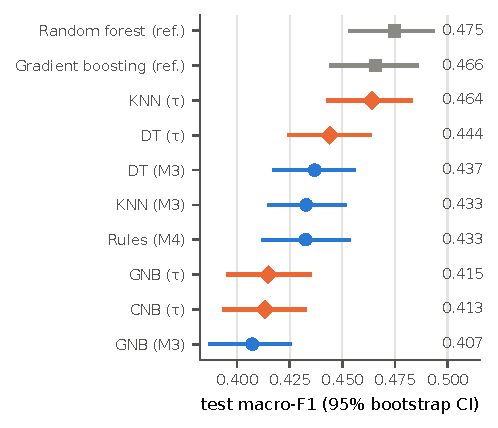
\includegraphics[width=0.97\linewidth]{m5_test_ci}
\caption{Test macro-F1 with 95\% CI. Circles: baselines; diamonds: extended; squares: reference ensembles.}\label{fig:ci}
\end{figure}

\subsection{What the trees say}\label{sec:tree}
The baseline tree splits first on size (\attr{n\_listings} $\leq103.5$), which accounts for 62\% of its impurity decrease, followed by price (13\%), share of new (7\%) and mileage (6\%). Its purest large leaf describes \emph{high} sellers: at most 17 listings, mileage below 79k, independent, not mainly sedans (279 sellers, 65\% \emph{high}; base rate 27\%).
The extended tree (16 leaves, \cref{fig:tree}) starts from an engineered attribute, the \emph{number of used cars} (63\% of the impurity decrease): size matters through the used stock more than through all listings. Read left to right, \emph{high} is predicted for sellers with few used cars, most purely with at most 17 and a savings/price ratio up to 10\% (1\,706 sellers, 49\% \emph{high}); \emph{medium} for expensive inventories (price $>36.2$k: 72--81\% \emph{medium}); \emph{low} for large, cheaper sellers ($>154$ listings and $>45$ used cars, 30\% \emph{low}), refined by price $\leq25.2$k in the next level (915 sellers, 37\% \emph{low} against 19\% overall, 35\% on the test set). Large leaves keep their precision on the test set (biggest leaf per class, train to test: \emph{high} 0.39 to 0.37, \emph{medium} 0.63 to 0.60, \emph{low} 0.37 to 0.35), small ones do not (47 sellers: 0.70 to 0.38). No leaf with more than 30 sellers is mostly \emph{low}: the data contain no clear profile of a low-rated seller.

\begin{figure*}[t]
\centering
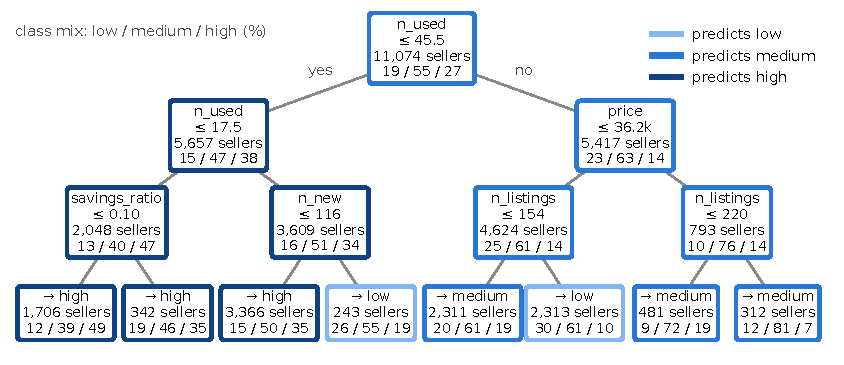
\includegraphics[width=0.97\textwidth]{m5_tree}
\caption{Extended Decision Tree, top three levels (left branch: condition true). Class mixes are unweighted shares of the training sellers; border: class predicted under the $\tau$-weighted rule.}\label{fig:tree}
\end{figure*}

\subsection{Error analysis: ordinality, ceiling, agreement}\label{sec:errors}
\paragraph{Ordinal errors} The rating is ordinal, so confusing \emph{low} and \emph{high} is worse than confusing neighbours. The baseline tree makes this error in 15\% of its mistakes, but the share must be read against chance: with the same marginals and independent predictions it would be 21\%. The ratio is 0.70--0.94 over all models, so they do capture the order, though weakly (QWK 0.14--0.26). The extended tree is best (12\% vs 17\% expected). We also tried an \textbf{ordinal decomposition} (Frank and Hall: two trees for $y>$ \emph{low} and $y>$ \emph{medium}, same grid): out-of-fold QWK 0.235 vs 0.233 and macro-F1 0.448 vs 0.445. Modelling the order explicitly adds nothing.

\paragraph{Ceiling} Extended KNN is statistically level with the ensembles, so a more flexible model does not extract much more from these attributes. The learning curves (\cref{fig:cross}, centre) are flattening but not flat: from 3\,500 to 8\,900 training sellers KNN gains only 0.013. More sellers would help slowly; better attributes are what is missing. A rating reflects service quality, and no column describes it.

\paragraph{By segment} The macro-F1 of the baseline tree is similar in the four K-Means segments (0.39--0.45): best in C1, worst in C3, where classes overlap most.

\paragraph{Agreement} Extended tree, extended KNN and the rule classifier, three different learners, agree on 52\% of the test sellers. Precision there is 0.58 overall, 0.68 on \emph{medium} (base rate 0.55), 0.48 on \emph{high} (0.27) and 0.39 on \emph{low} (0.19); where they disagree KNN is right in 45\% of the cases. Agreement is a usable confidence signal, but even three concordant models are often wrong on \emph{low}.

\begin{figure*}[t]
\centering
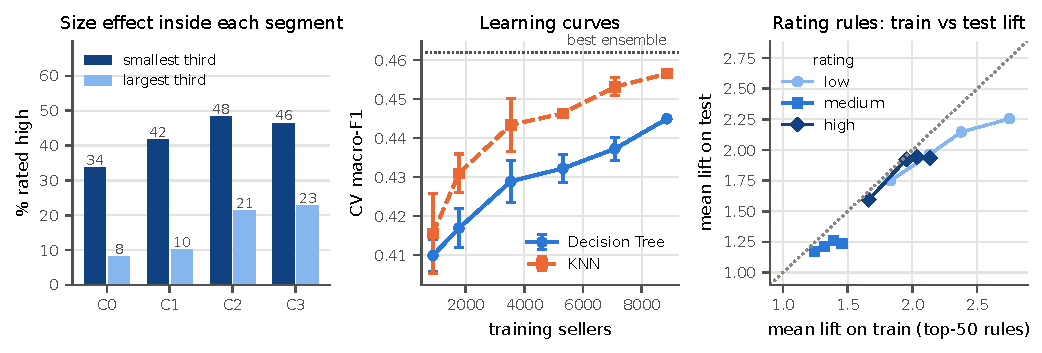
\includegraphics[width=0.95\textwidth]{m5_cross_module}
\caption{Left: share of \emph{high} among the smallest and largest third of the sellers of each K-Means segment. Centre: learning curves of the extended models. Right: lift of the 50 best rating rules per support band, train vs test (dotted: identity; see \cref{sec:exploit}).}\label{fig:cross}
\end{figure*}

\subsection{Seller size confounds dealer type}\label{sec:simpson}
\begin{table}[t]
\centering
\caption{Rating vs size. Top: Spearman's $\rho_s$ between \attr{n\_listings} and rating, and shares among the smallest (S) and largest (L) third of each group. Bottom: dealer type within size tertiles.}\label{tab:size}
\tab{m5_size}\\[5pt]
\tab{m5_dealer}
\end{table}

\Cref{sec:m1,sec:m2} found that independents are rated \emph{high} more often than franchises (33\% vs 21\%). Is this dealer type or size? The \textbf{size effect is universal}: within every segment and both dealer types small sellers are \emph{high} 2 to 4 times as often as large ones (\cref{tab:size}, top; \cref{fig:cross}, left). The \textbf{dealer effect reverses}: in no size tertile do independents have more \emph{high} sellers, and among mid and large ones franchises have clearly more (\cref{tab:size}, bottom). The crude odds ratio of \emph{high} for franchises is 0.53 (95\% CI 0.49--0.57); adjusted for size deciles (Mantel--Haenszel) it becomes \textbf{1.73} (1.54--1.95). This is a Simpson's paradox: independents look better because they are small (median 26 vs 154 listings). It corrects the naive reading of \cref{fig:target} and explains why the tree needs size first.

\subsection{Regression}\label{sec:reg}
\paragraph{Task} The target is \attr{price} (seller median), on the \code{log1p} scale: it is the central economic attribute, is strongly related to the others, and its log is almost symmetric (skew $3.4\to-0.4$), so additive effects become relative ones. No predictor derives from price. Split and folds are those of the classification; tuning minimizes CV MSE.

\paragraph{Single regression} On the training set \attr{mileage} has the strongest correlation with price ($\rho_s=-0.82$) and is the textbook driver of used-car prices. OLS gives $\widehat{\log(1+\mathrm{price})}=10.40-0.1035\,\mathrm{mileage}/10^4$: about $-9.8\%$ per 10\,000 miles. It explains 75\% of the variance on train and test alike, but only 48\% in dollars. The residuals (\cref{fig:slr}) show where the line fails: new-car sellers pile up at zero mileage with any price, nearly new stock (100--20k miles) is under-predicted ($+0.09$), and the spread grows with mileage (std 0.25 to 0.42).

\begin{figure*}[t]
\centering
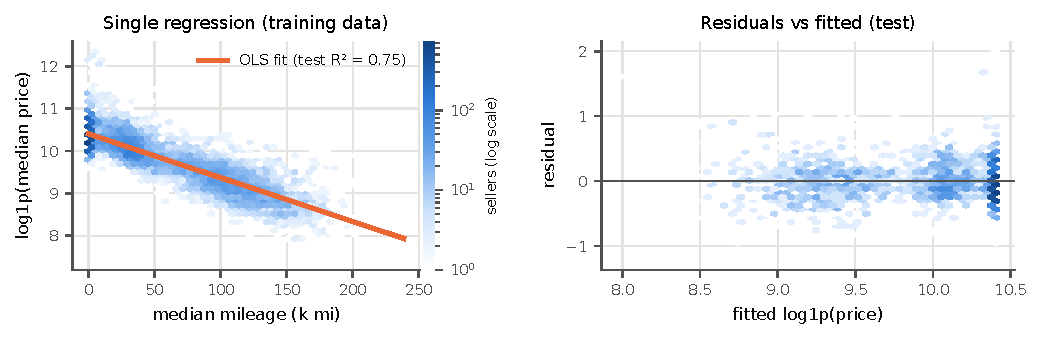
\includegraphics[width=0.93\textwidth]{m3_slr}
\caption{Single regression of log price on mileage: fit on the training set (left), test residuals (right).}\label{fig:slr}
\end{figure*}

\paragraph{Multiple regression} Four predictors cover different aspects: \attr{mileage} (wear), \attr{horsepower}, \attr{width} (vehicle class) and \attr{pct\_is\_new} (composition); all VIFs are below 2.5. We compare OLS with two non-linear models: a Decision Tree regressor (depth $\{2,3,4,5,6,8,10,12,15,\text{none}\}$ $\times$ leaf $\{1,5,10,20,50,100\}$, 60 configurations; best depth 12, leaf 20, CV MSE 0.0374; e.g.\ 0.048 at depth 5) and KNN on standardized inputs ($k\in\{1,3,5,7,10,15,20,30,50,75,100\}$ $\times$ $p\in\{1,2\}$ $\times$ weights, 44 configurations; best $k=30$, $p=1$, distance weights, CV MSE 0.0337). \Cref{tab:reg,fig:regpred}: three more predictors halve the linear error ($R^2$ 0.747 to 0.876). In the standardized OLS, mileage ($-0.48$) and horsepower ($+0.21$) carry nearly all the effect. The non-linear models add 0.03--0.04 of $R^2$ by modelling the zero-mileage regime and interactions; KNN has the lowest test error, the tree a smaller model that can be read. KNN's zero training error is again an effect of distance weights.

\begin{table}[t]
\centering
\caption{Regression on log price (same split and target). $R^2$(\$): after back-transformation to dollars.}\label{tab:reg}
\tabtight{m3_reg}
\end{table}

\begin{figure*}[t]
\centering
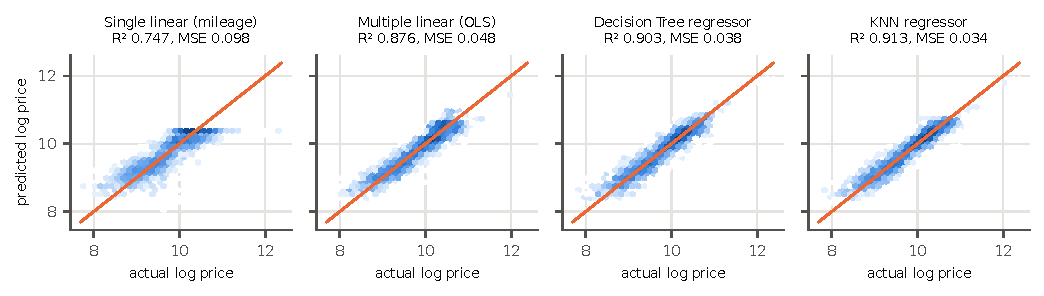
\includegraphics[width=0.95\textwidth]{m3_regression_pred}
\caption{Predicted vs actual log price on the test set.}\label{fig:regpred}
\end{figure*}

\paragraph{Sensitivity} \Cref{tab:regabl} crosses three predictor sets with the target scale (training-set CV). On the raw scale OLS predicts \emph{negative} prices for 107--206 sellers and, judged on the log scale, is worse than the mean: the log target is essential for linear models and irrelevant for tree and KNN. With all 18 numerical predictors OLS and the tree improve (CV $R^2$ 0.880 to 0.896 and 0.903 to 0.910), KNN does not (0.913 to 0.914). On the test set the 18-predictor models give 0.896 (OLS), 0.910 (tree) and 0.908 (KNN), so none beats KNN on four attributes (0.913). Four interpretable predictors are enough.

\begin{table}[t]
\centering
\caption{Regression ablation, training-set CV: 1 (mileage), 4 or 18 predictors. APE: median absolute percentage error; neg.: negative predicted prices.}\label{tab:regabl}
\tabtight{m5_reg}
\end{table}

\subsection{Which algorithms are best?}\label{sec:best}
\Cref{tab:best} compares the classifiers from several perspectives.

\begin{table}[t]
\centering
\caption{Classifiers by perspective (extended models, test set).}\label{tab:best}
{\tabfont\setlength{\tabcolsep}{2.5pt}
\begin{tabular}{@{}p{0.20\linewidth}p{0.24\linewidth}p{0.24\linewidth}p{0.22\linewidth}@{}}
\toprule
 & Decision Tree & KNN & Na\"ive Bayes\\
\midrule
\Fm\ / AUC & 0.444 / 0.634 & \textbf{0.464 / 0.658} & 0.415 / 0.609\\
CV--test gap & $<0.001$ & 0.008 & 0.008\\
Readability & \textbf{16 rules} & none & likelihoods\\
Skew, outliers & \textbf{invariant} & log, scaling & log or bins\\
Assumptions & none & meaningful distance & independence: violated\\
Cost & \textbf{negligible} & 11k distances per query & negligible\\
\bottomrule
\end{tabular}}
\end{table}

\paragraph{Classification} \textbf{KNN} ($k=151$, $\tau=0.8$) is the best predictor: it leads macro-F1, accuracy and AUC, in CV as on the test set, and is statistically level with the ensembles. The \textbf{Decision Tree} is close, explains itself and costs nothing: it is the model to show to a user, and it has the best ordinal agreement among the lecture models (QWK 0.26). On the baseline grids alone the two are tied and the tree would be preferred. Na\"ive Bayes pays for correlated attributes.

\paragraph{Regression} KNN has the lowest error ($R^2$ 0.913), the Decision Tree regressor (0.903) offers the best trade-off with a small train--test gap (MSE 0.028 vs 0.038), and OLS (0.876) is the most interpretable. Price is strongly determined by the inventory, the rating only weakly.

